\begin{exercise}
\begin{figure}[H]
\centering
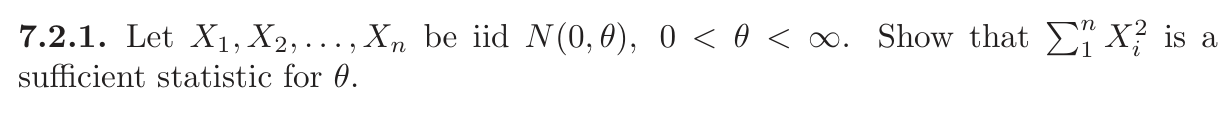
\includegraphics[width=\textwidth]{hw11-2025051819.png}
% \caption{}
\label{}
\end{figure}
\end{exercise}
\[
Y\coloneqq \sum_{i=1}^{n} X_i^2
\]
\[
\frac{1}{\sqrt{ \theta }}X_i\sim N(0,1)\Rightarrow\frac{X_i^2}{\theta}\sim \chi^{2}(1)\Rightarrow \frac{Y}{\theta}=\sum_{i=1}^{n} \frac{X_i^2}{\theta}\sim \chi^{2}(n)
\]
\[
\prod_{i=1}^{n} f_{X_i}(x_i;\theta)=\prod_{i=1}^{n} \frac{1}{\sqrt{ 2\pi\theta }}\exp \left\{  -\frac{x_i^2}{2\theta}  \right\}=(2\pi\theta)^{-\frac{n}{2}}\exp \left\{  -\frac{1}{2\theta}\sum_{i=1}^{n} x_i^2  \right\}
\]
\[
\begin{aligned}
f_{Y}(y;\theta) & =\frac{ \partial   }{ \partial y } \mathbb{P}(Y\leq y) \\
 & =\frac{ \partial   }{ \partial y } \mathbb{P}\left( \frac{Y}{\theta}\leq \frac{y}{\theta} \right) \\
 & =\frac{1}{\theta}f_{\frac{Y}{\theta}}(y;\theta) \\
 & =\frac{1}{\theta}\cdot\frac{1}{\Gamma\left( \frac{n}{2} \right)2^{n/2}}\cdot \left( \frac{y}{\theta} \right)^{n/2-1}\exp \left\{  -\frac{y}{2\theta}  \right\} \\
 & =\frac{1}{\Gamma\left( \frac{n}{2} \right)2^{n/2 }}\frac{1}{\theta^{n/2 }}y^{n/2-1 }\exp \left\{  -\frac{y}{2\theta}  \right\}
\end{aligned}
\]
Let $y=\sum_{i=1}^{n}x_i^2$ then
\[
f_{Y}\left( \sum_{i=1}^{n} x_i^2 ;\theta\right)=\frac{1}{\Gamma\left( \frac{n}{2} \right)2^{n/2 }}\frac{1}{\theta^{n/2 }}\left( \sum_{i=1}^{n} x_i^2  \right)^{n/2-1 }\exp \left\{  -\frac{\sum_{i=1}^{n} x_i^2}{2\theta}  \right\}
\]
Then
\[
\frac{\prod_{i=1}^{n} f_{X_i}(x_i;\theta)}{f_{Y}(y;\theta)}=\frac{\Gamma\left( \frac{n}{2} \right)}{\pi^{-\frac{n}{2}}}\left( \sum_{i=1}^{n} x_i^2 \right)^{n/2-1}
\]
does not depend on $\theta$. Thus $Y$ is sufficient.

\begin{exercise}
\begin{figure}[H]
\centering
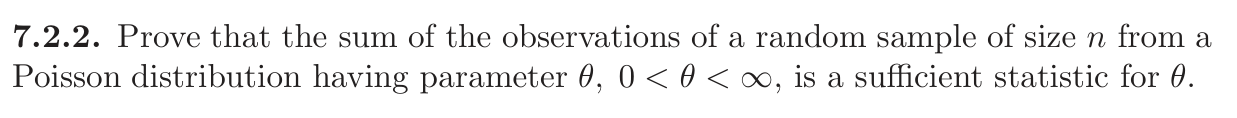
\includegraphics[width=\textwidth]{1-hw11-2025051819.png}
% \caption{}
\label{}
\end{figure}
\end{exercise}
\[
X_i\sim \text{Poi}(\theta)
\]
\[
Y\coloneqq \sum_{i=1}^{n} X_i\sim \text{Poi}(n\theta)
\]
Then
\[
\frac{\prod_{i=1}^{n} f_{X_i}(x_i;\theta)}{f_{Y}\left( \sum_{i=1}^{n} x_i;\theta \right)}=\frac{\left( \sum_{i=1}^{n} x_i \right)!}{x_1!\dots x_n!}\cdot n^{-\sum_{i=1}^{n} x_i}
\]
does not depend on $\theta$. Thus $Y$ is sufficient.

\begin{exercise}
\begin{figure}[H]
\centering
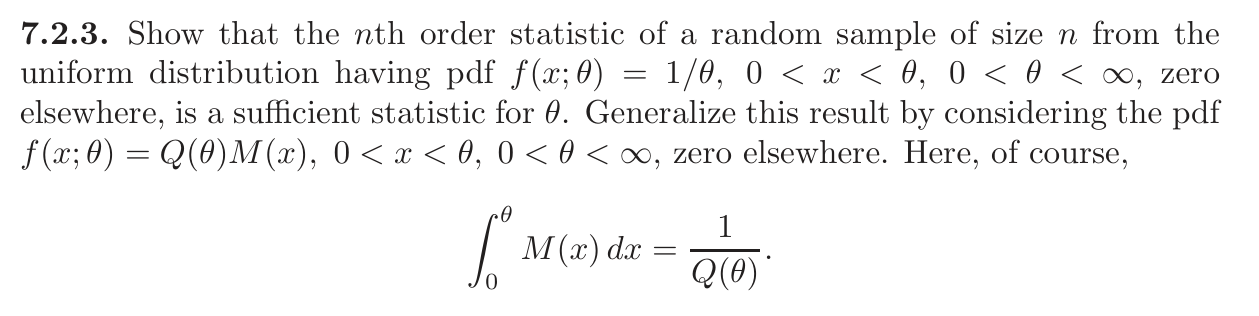
\includegraphics[width=\textwidth]{2-hw11-2025051819.png}
% \caption{}
\label{}
\end{figure}
\end{exercise}
For $X_i\sim U(0,\theta)$,
\[
\frac{\prod_{i=1}^{n} f_{X_i}(x_i;\theta)}{f_{X_{(n)}}(x_{(n)};\theta)}=\frac{\theta^{-n}\cdot \mathbb{1}_{x_{(n)}<\theta}}{n\theta^{-n}x_{(n)}^{n-1}\cdot \mathbb{1}_{x_{(n)}<\theta}}=\frac{1}{n\cdot x^{n-1}_{(n)}}
\]
does not depend on $\theta$. Thus $X_{(n)}$ is sufficient.

In the general case,
\[
\begin{aligned}
\frac{\prod_{i=1}^{n} f_{X_i}(x_i;\theta)}{f_{X_{(n)}}(x_{(n)};\theta)} & =\frac{\left[ \prod_{i=1}^{n} M(x_i) \right]\cdot[Q(\theta)]^{n}\cdot \mathbb{1}_{x_{(n)}<\theta}}{n\cdot\left[ \int_{0}^{x_{(n)}} Q(\theta)M(s) \, \mathrm{d}s  \right]^{n-1}\cdot Q(\theta) M(x_{(n)})\cdot \mathbb{1}_{x_{(n)}<\theta}} \\
 & =\frac{\prod_{i=1}^{n} M(x_i)}{n\cdot\left[ \int_{0}^{x_{(n)}} M(s) \, \mathrm{d}s  \right]^{n-1}\cdot M(x_{(n)})}
\end{aligned}
\]
does not depend on $\theta$. Thus $X_{(n)}$ is sufficient.

\begin{exercise}
\begin{figure}[H]
\centering
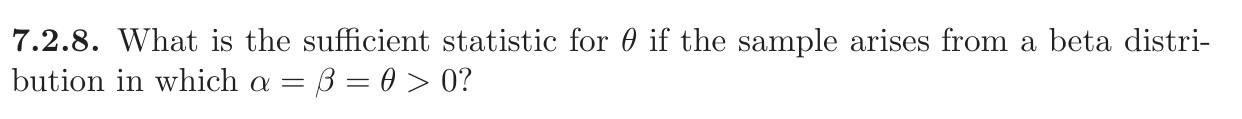
\includegraphics[width=\textwidth]{3-hw11-2025051819.png}
% \caption{}
\label{}
\end{figure}
\end{exercise}
\[
X_i\sim \text{beta}(\theta,\theta)
\]
\[
f_{X_i}(x;\theta)=\frac{\Gamma(2\theta)}{\Gamma(\theta)\Gamma(\theta)}(x(1-x))^{\theta-1}
\]
Then the Likelihood function is
\[
\prod_{i=1}^{n} f_{X_i}(x_i;\theta)=\prod_{i=1}^{n} \frac{\Gamma(2\theta)}{(\Gamma(\theta))^2}(x_i(1-x_i))^{\theta-1}=\frac{(\Gamma(2\theta))^{n}}{(\Gamma(\theta))^{2n}}\prod_{i=1}^{n} (x_i(1-x_i))^{\theta-1}
\]
By Neyman Factorization Theorem,
\[
T=\prod_{i=1}^{n} X_i(1-X_i)
\]
is the sufficient statistic for $\theta$.

\begin{exercise}
\begin{figure}[H]
\centering
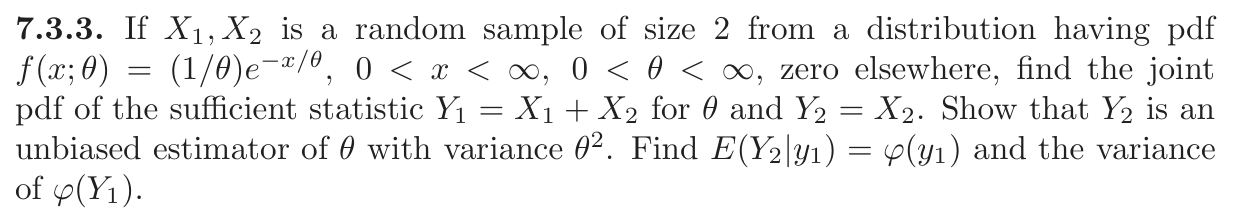
\includegraphics[width=\textwidth]{5-hw11-2025051819.png}
% \caption{}
\label{}
\end{figure}
\end{exercise}
\[
\mathbb{E}(Y_2)=\mathbb{E}(X_2)=\int_{0}^{\infty} x\cdot\frac{1}{\theta}\exp \left\{  -\frac{x}{\theta}  \right\} \, \mathrm{d}x =\theta
\]
\[
\begin{aligned}
\mathrm{Var}(Y_2) & =\mathrm{Var}(X_2) \\
 &  =\mathbb{E}(X_2^2)-(\mathbb{E}(X_2))^2\\
 & =\int_{0}^{\infty} x^2\cdot\frac{1}{\theta}\exp \left\{  -\frac{x}{\theta}  \right\} \, \mathrm{d}x -(\mathbb{E}(X_2))^2  \\
 & =2\theta^{2}-\theta^{2} \\
 & =\theta^{2}
\end{aligned}
\]
\[
\mathbb{E}(Y_2|Y_1=y_1)=\int_{}^{} y_2f_{Y_2|Y_1}(y_2|y_1) \, \mathrm{d}y_2 
\]
\[
f_{Y_2|Y_1}(y_2|y_1)=\frac{f_{Y_1,Y_2}(y_1,y_2)}{f_{Y_1}(y_1)}
\]
\[
f_{X_1,X_2}(x_1,x_2)=\frac{1}{\theta^{2}}e^{ -(x_1+x_2)/\theta }\qquad 0<x_1,x_2<\infty
\]
\[
f_{Y_1,Y_2}(y_1,y_2)=f_{X_1,X_2}(y_1-y_2,y_2)\begin{vmatrix}
1 & -1 \\
0 & 1 
\end{vmatrix}=\frac{1}{\theta^{2}}e^{ -y_1/\theta }\qquad 0<y_2<y_1<\infty
\]
\[
f_{Y_1}(y_1)=\int_{0}^{y_1} f_{Y_1,Y_2}(y_1,y_2) \, \mathrm{d}y_2 =\frac{y_1}{\theta^{2}}e^{ -y_1/\theta }
\]
\[
f_{Y_2|Y_1}(y_2|y_1)=\frac{f_{Y_1,Y_2}(y_1,y_2)}{f_{Y_1}(y_1)}=\frac{1}{y_1}\qquad 0<y_2<y_1
\]
\[
\begin{aligned}
\mathbb{E}(Y_2|Y_1=y_1) & =\int_{}^{} y_2f_{Y_2|Y_1}(y_2|y_1) \, \mathrm{d}y_2  \\
 & =\int_{}^{} y_2 \frac{1}{y_1} \, \mathrm{d}y_2 \\
 & =\frac{y_1}{2}
\end{aligned}
\]
\[
\varphi(y_1)=\frac{y_1}{2}
\]
\[
\mathbb{E}(\varphi(Y_1))=\frac{1}{2}\mathbb{E}Y_1=\frac{1}{2}\int_{0}^{\infty} y_1\cdot\frac{y_1}{\theta^{2}}e^{ -y_1/\theta } \, \mathrm{d}y_1=\theta
\]
\[
\mathbb{E}((\varphi(Y_1))^2)=\frac{1}{4}\mathbb{E}(Y_1^2)=\frac{1}{4}\int_{0}^{\infty} y_1^2\cdot\frac{y_1}{\theta^{2}} e^{ -y_1/\theta }\, \mathrm{d}y_1=\frac{3}{2}\theta^{2}
\]
\[
\mathrm{Var}(\varphi(Y_1))=\mathbb{E}((\varphi(Y_1))^2)-(\mathbb{E}(\varphi(Y_1)))^2=\frac{\theta^{2}}{2}
\]
\begin{exercise}
\begin{figure}[H]
\centering
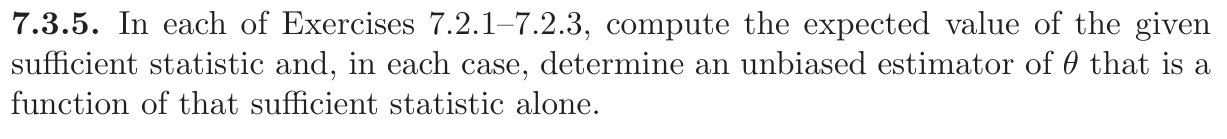
\includegraphics[width=\textwidth]{6-hw11-2025051819.png}
% \caption{}
\label{}
\end{figure}
\end{exercise}
7.2.1
\[
Y\coloneqq \sum_{i=1}^{n} X_i^2
\]
\[
\frac{1}{\theta}Y=\sum_{i=1}^{n} \left( \frac{X_i}{\sqrt{ \theta }} \right)^2\sim \chi^{2}(n)
\]
\[
\begin{aligned}
\mathbb{E}(Y) & =\theta \cdot\mathbb{E}\left( \frac{Y}{\theta} \right) \\
 & =\theta \int_{0}^{\infty}x\cdot \frac{1}{\Gamma\left( \frac{n}{2} \right)2^{n/2 }}x^{n/2-1 }e^{ -\frac{x}{2} } \, \mathrm{d}x  \\
 & =\theta \int_{0}^{\infty} \frac{1}{\Gamma\left( \frac{n}{2} \right)2^{n/2 }}x^{\frac{n}{2} }e^{ -\frac{x}{2} } \, \mathrm{d}x \\
 & =\frac{\theta}{\Gamma\left( \frac{n}{2} \right)}\int_{0}^{\infty} \left( \frac{x}{2} \right)^{\frac{n}{2}}e^{ -\frac{x}{2} } \, \mathrm{d}x  \\
 & =\frac{2\theta}{\Gamma\left( \frac{n}{2} \right)} \underbrace{ \int_{0}^{\infty} x^{\frac{n}{2}}e^{ -x } \, \mathrm{d}x }_{ =\Gamma\left( \frac{n}{2}+1 \right) }  \\
 & =n\theta
\end{aligned}
\]
The unbiased sufficient estimator is
\[
\frac{1}{n}\sum_{i=1}^{n} X_i^2
\]
7.2.2
\[
Y\coloneqq \sum_{i=1}^{n} X_i\sim \text{Poi}(n\theta)
\]
\[
\mathbb{E}(Y)=\sum_{k=0}^{\infty} \frac{k\cdot(n\theta)^{k}e^{ -n\theta }}{k!}=\sum_{k=1}^{\infty} \frac{(n\theta)^{k}e^{ -n\theta }}{(k-1)!}=n\theta \cdot \sum_{k=0}^{\infty } \frac{(n\theta)^{k}e^{ -n\theta }}{k!}=n\theta
\]
The unbiased sufficient estimator is
\[
\frac{1}{n}\sum_{i=1}^{n} X_i
\]
7.2.3
\[
f_{X_{(n)}}(x)=n\theta^{-n}x^{n-1}\cdot \mathbb{1}_{x<\theta}
\]
\[
\mathbb{E}(X_{(n)})=\int_{0}^{\theta} x\cdot n\theta^{-n}x^{n-1} \, \mathrm{d}x =\frac{n}{n+1}\theta
\]
The unbiased sufficient estimator is
\[
\frac{n+1}{n}X_{(n)}
\]
\begin{exercise}
\begin{figure}[H]
\centering
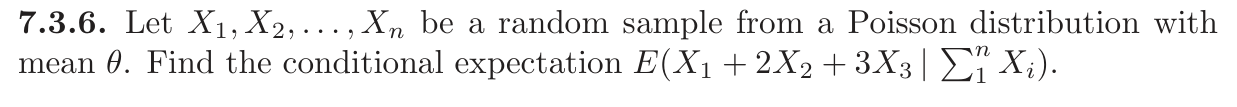
\includegraphics[width=\textwidth]{7-hw11-2025051819.png}
% \caption{}
\label{}
\end{figure}
\end{exercise}
\[
X_i\sim \text{Poi}(\theta)
\]
\[
\begin{aligned}
 & \quad  \mathbb{E}\left( X_1+2X_2+3X_3|\sum_{i=1}^{n}X_i  \right) \\
 & =\mathbb{E}\left( X_1|\sum_{i=1}^{n} X_i \right)+2\mathbb{E}\left( X_2|\sum_{i=1}^{n} X_i \right)+3\mathbb{E}\left( X_3|\sum_{i=1}^{n} X_i \right) \\
 & =6\mathbb{E}\left( X_1|\sum_{i=1}^{n} X_i \right) 
\end{aligned}
\]
Denote
\[
Y_1=\sum_{i=1}^{n} X_i,\quad Y_2=X_1,\quad Y_k=X_k,\quad k=3,\dots,n
\]
Then
\[
\mathbb{E}\left( X_1|\sum_{i=1}^{n} X_i \right)=\mathbb{E}(Y_2|Y_1)=\sum_{y_2=0}^{Y_1} y_2f_{Y_2|Y_1}(y_2|y_1)
\]
\[
f_{Y_2|Y_1}(y_2|y_1)=\frac{f_{Y_1,Y_2}(y_1,y_2)}{f_{Y_1}(y_1)}
\]
\[
\begin{aligned}
 & \quad f_{Y_1,\dots,Y_n}(y_1,\dots ,y_n) \\
 & =f_{X_1,\dots,X_n}\left( y_2,y_1-\sum_{i=2}^{n} y_i,y_3,\dots,y_n \right)\underbrace{ \begin{Vmatrix}
0 & 1 & 0 & 0 & \dots & 0 \\
1 & -1 & -1 & -1 & \dots & -1 \\
0 & 0 & 1 & 0 & \dots & 0 \\
\vdots & \vdots & \vdots & \ddots & \ddots & \vdots \\
0 & 0 & 0 & 0 & 1 & 0 \\
0 & 0 & 0 & 0 & 0 & 1
\end{Vmatrix} }_{ =1 } \\
 & =f_{X_1,\dots,X_n}\left( y_2,y_1-\sum_{i=2}^{n} y_i,y_3,\dots,y_n \right) \\
 & =\frac{\theta^{y_1-\sum_{i=2}^{n} y_i }e^{ -\theta }}{\left( y_1-\sum_{i=2}^{n} y_i \right)!}\cdot \prod_{i=2}^{n} \frac{\theta^{y_i}e^{ -\theta } }{y_i!} \\
 & =e^{ -n\theta }\cdot\frac{\theta^{y_1}}{\left( y_1-\sum_{i=2}^{n} y_i \right)!\cdot y_2!\dots  y_n!}
\end{aligned}
\]
We have the identity:
\[
\sum_{k=0}^{m} \frac{s^{m-k}}{k!\cdot(m-k)!}=\frac{1}{m!}\sum_{k=0}^{m}{\binom{m}{k} } s^{m-k}=\frac{1}{m!}(1+s)^{m}
\]
Thus
\[
\begin{aligned}
f_{Y_1,Y_2}(y_1,y_2) & =\sum_{y_3,\dots,y_n}f_{Y_1,\dots,Y_n}(y_1,\dots ,y_n) \\
 & =\sum_{y_n=0}^{y_1-y_2} \sum_{y_{n-1}=0}^{y_1-y_2-y_n} \dots \sum_{y_3=0}^{y_1-y_2-\sum_{i=4}^{n} y_i} f_{Y_1,\dots,Y_n}(y_1,\dots ,y_n) \\
 & =\sum_{y_n=0}^{y_1-y_2} \sum_{y_{n-1}=0}^{y_1-y_2-y_n} \dots \sum_{y_3=0}^{y_1-y_2-\sum_{i=4}^{n} y_i}\theta^{y_1}e^{ -n\theta }\cdot\frac{1}{\left( y_1-\sum_{i=2}^{n} y_i \right)!\cdot y_2!\cdot y_3!\dots  y_n!} \\
 & =\sum_{y_n=0}^{y_1-y_2} \sum_{y_{n-1}=0}^{y_1-y_2-y_n} \dots \sum_{y_4=0}^{y_1-y_2-\sum_{i=5}^{n} y_i}\theta^{y_1}e^{ -n\theta }\cdot\frac{2^{y_1-y_2-\sum_{i=4}^{n} y_i}}{\left( y_1-y_2-\sum_{i=4}^{n} y_i \right)!\cdot y_2!\cdot y_4!\dots  y_n!} \\
 & =\dots \\
 & =\theta^{y_1}e^{ -n\theta }\frac{(n-1)^{y_1-y_2}}{(y_1-y_2)!\cdot y_2!}\qquad 0<y_2\leq y_1<\infty
\end{aligned}
\]
\[
f_{Y_1}(y_1)=\theta^{y_1}e^{ -n\theta }\sum_{y_2=0}^{y_1} \frac{(n-1)^{y_1-y_2}}{y_2!\cdot(y_1-y_2)!}=\theta^{y_1}e^{ -n\theta }\cdot\frac{1}{y_1!}\cdot n^{y_1}=\frac{e^{ -n\theta }(n\theta)^{y_1}}{y_1!}
\]
Therefore
\[
\begin{aligned}
f_{Y_2|Y_1}(y_2|y_1) & =\frac{f_{Y_1,Y_2}(y_1,y_2)}{f_{Y_1}(y_1)} \\
 & =\frac{\theta^{y_1}e^{ -n\theta }\frac{(n-1)^{y_1-y_2}}{(y_1-y_2)!\cdot y_2!}}{\frac{e^{ -n\theta }(n\theta)^{y_1}}{y_1!}} \\
 & =\frac{(n-1)^{y_1-y_2}\cdot y_1!}{n^{y_1}(y_1-y_2)!\cdot y_2!} \\
 & =\binom{y_1}{y_2} \frac{(n-1)^{y_1-y_2}}{n^{y_1}}\qquad 0<y_2\leq y_1<\infty
\end{aligned}
\]
\[
\mathbb{E}\left( X_1|\sum_{i=1}^{n} X_i \right)=\mathbb{E}(Y_2|Y_1)=\sum_{y_2=0}^{y_1} y_2\binom{y_1}{y_2} \frac{(n-1)^{y_1-y_2}}{n^{y_1}}
\]
We have the identity
\[
(1+p)^{n}=\sum_{k=0}^{n}\binom{n}{k} p^{k}
\]
\[
n(1+p)^{n-1}=\sum_{k=0}^{n} \binom{n}{k} kp^{k-1}
\]
Then
\[
\begin{aligned}
\mathbb{E}\left( X_1|\sum_{i=1}^{n} X_i \right) & =\sum_{y_2=0}^{y_1} y_2\binom{y_1}{y_2} \frac{(n-1)^{y_1-y_2}}{n^{y_1}} \\
 & =\left( \frac{n-1}{n} \right)^{y_1}\sum_{y_2=0}^{y_1} y_2\binom{y_1}{y_2} \left( \frac{1}{n-1} \right)^{y_2} \\
 & =\left( \frac{n-1}{n} \right)^{y_1}\cdot\frac{1}{n-1}\cdot y_1\left( 1+\frac{1}{n-1} \right)^{y_1-1} \\
 & =\frac{y_1}{n} \\
 & =\frac{1}{n}\sum_{i=1}^{n} X_i
\end{aligned}
\]
Hence
\[
\mathbb{E}\left( X_1+2X_2+3X_3|\sum_{i=1}^{n}X_i  \right)=\frac{6}{n}\sum_{i=1}^{n} X_i
\]